\documentclass{beamer}
\usepackage[utf8]{inputenc}
\usepackage[ngerman]{babel}
\usepackage{amsmath}
\usepackage{amsfonts}
\usepackage{amssymb}
\usepackage{graphicx} 
\usepackage{float}
\usepackage{listings} 
\usepackage{xcolor}
\usepackage[backend=bibtex,style=numeric,citestyle=verbose]{biblatex}
\usepackage{graphicx}
\usepackage{caption}
\usepackage{subcaption}
\usepackage[automark]{scrpage2}
\usepackage[stable]{footmisc}
\usepackage{pgfpages}

\bibliography{presentation}
\usetheme{Berlin}
\usecolortheme{dolphin}
\beamertemplatenavigationsymbolsempty
\setbeameroption{show notes on second screen}
% \setbeameroption{hide notes}
\begin{document}
\title{On the relationships between QoS and software adaptability at the architectural level}
\author{Daniel Schmidt}
\date{17.02.2015}

\frame{\titlepage}

\frame{\frametitle{Inhalt}\tableofcontents}

\section{Einleitung}
\frame{\frametitle{Einleitung}

\begin{figure}[h]
\centering
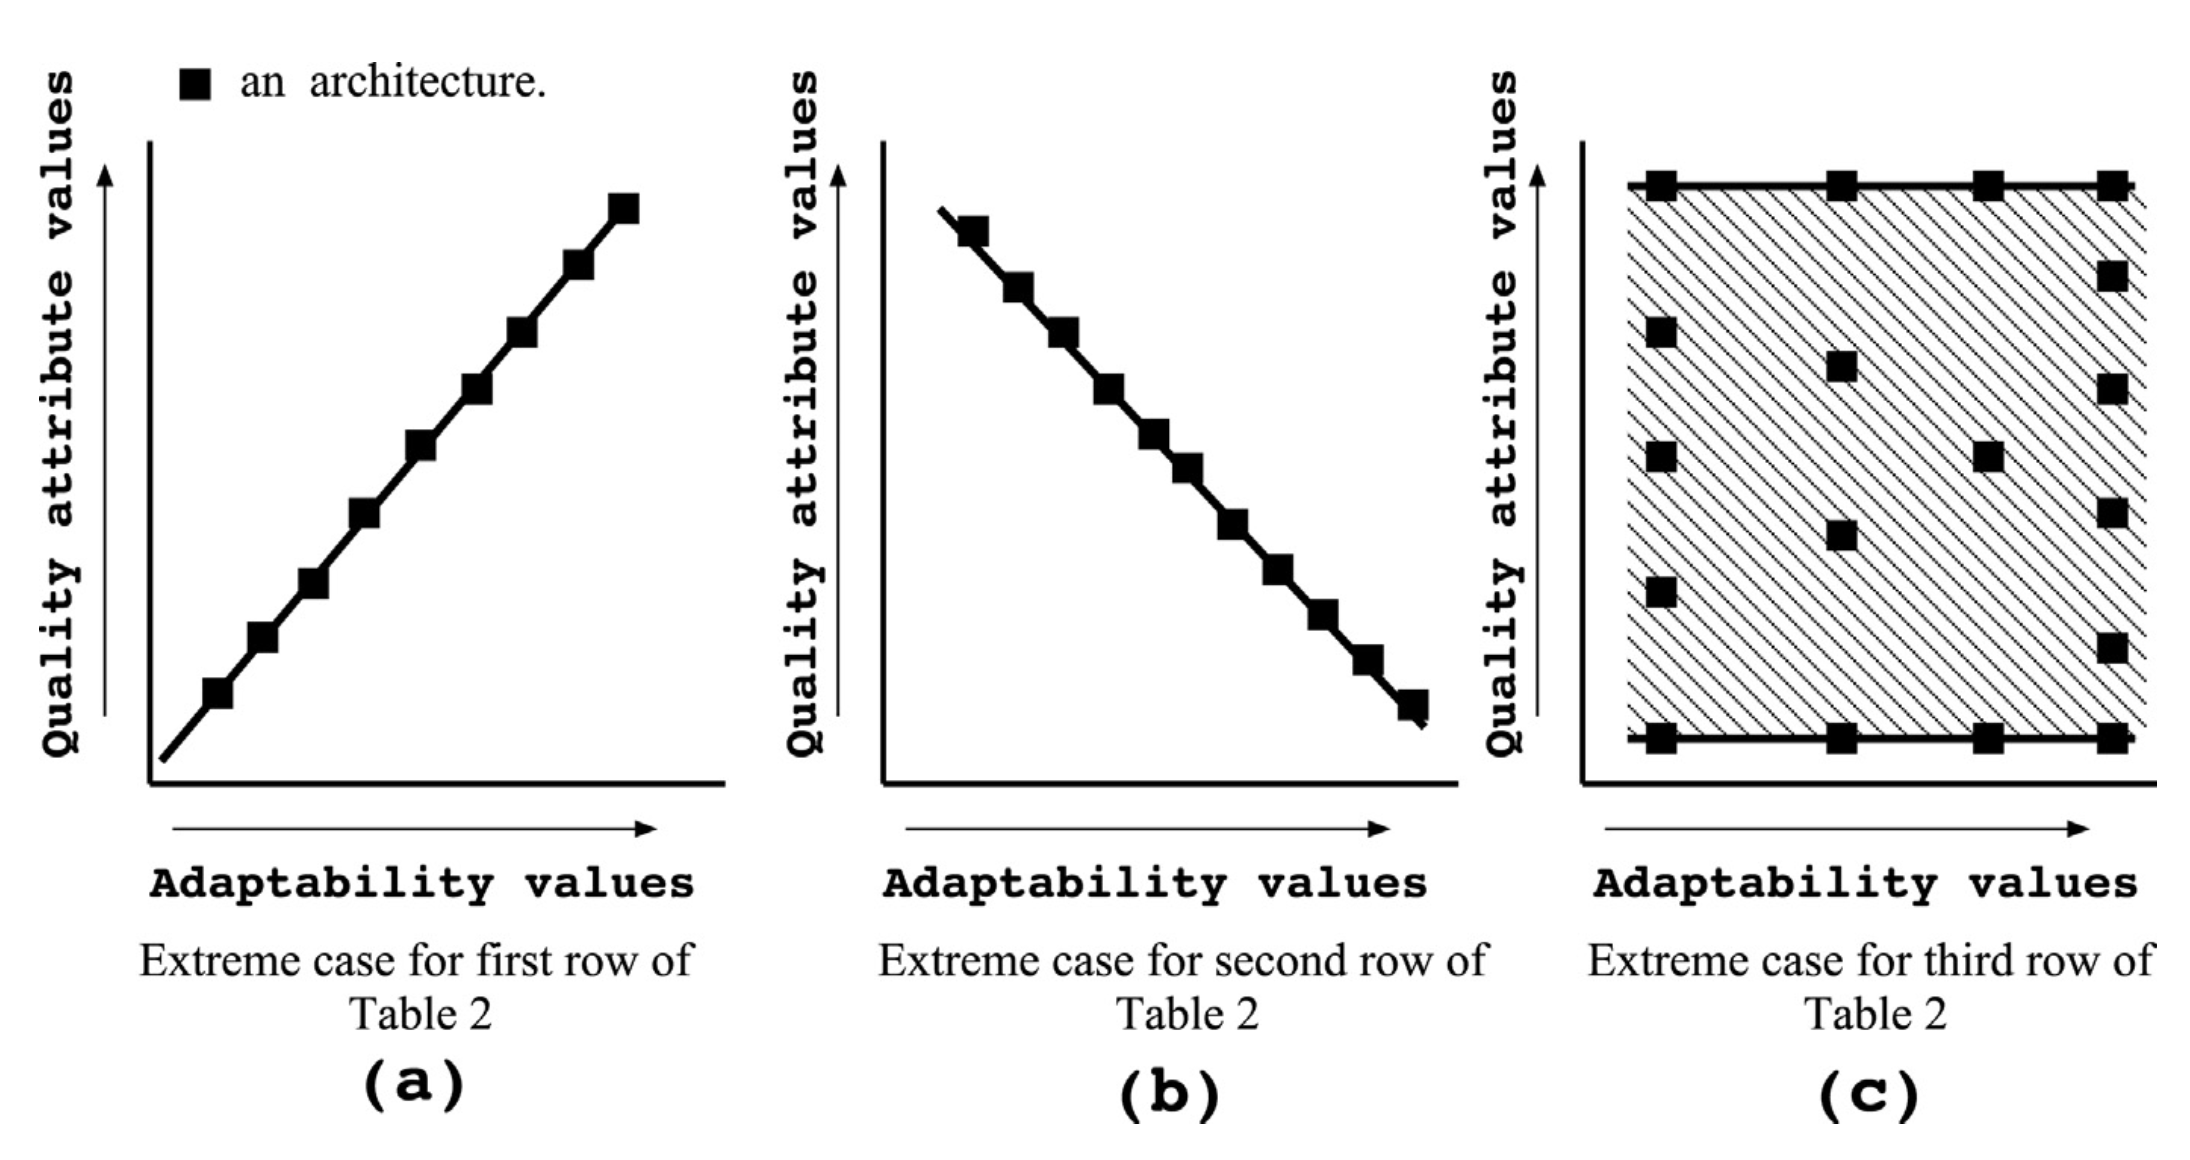
\includegraphics[width=\textwidth]{img/fig3.png}
\caption{Zusammenhang zwischen Anpassungsfähigkeit und QoS}
\end{figure}

\note{
\begin{itemize}
\item Es geht immer um garantierte Anpassungsfähigkeit
\item Garantierte Anpassungsfähigkeit von Software kann andere Qualitätsattribute wie Geschwindigkeit, Verlässlichkeit und Wartbarkeit beeinflussen.
\item Ansatz ist bei einem wechselnden Kontext nützlich, er wird benutzt um zu testen ob die ausgewählten Komponenten die Voraussetzungen des Systems erfüllen.
\end{itemize}
}
}

\section{Anpassungsfähigkeit}
\frame{\frametitle{Anpassungsfähigkeit} 

\begin{Definition}[Anpassungsfähiges Software System]
Ein anpassungsfähiges Software System kann Änderungen in der Umwelt ohne einen externen Eingriff vertragen.
\end{Definition}
\tiny{\cite{def-adaptability}}

\note {
\begin{itemize}
\item  Quantifizierung des Grads der Anpassungsfähigkeit wichtig
\item Über heuristische Verfahren kann eine automatische Anpassung der Architektur erfolgen, hin zu einer Architektur, welche die Qualitätsmerkmale erfüllt oder nah dran ist
\item Die Ziele des Papers sind: \begin{itemize}
	\item Eine erweiterte Menge von architekturellen Metriken die zur Evaluierung der Anpassungsfähigkeit des Systems verwendet werden können
	\item Der Ansatz benutzt diese Metriken um die Beziehung zwischen Anpassungsfähigkeit und Qualitätswerten zu definieren, damit hilft dieser Ansatz bei der Begründung des Designs
	\item Ein Hilfsmittel bereitstellen um den Ansatz zu benutzen
\end{itemize}
\end{itemize}
}
}
\frame{\frametitle{Beispiel}

\begin{figure}[h]
\centering
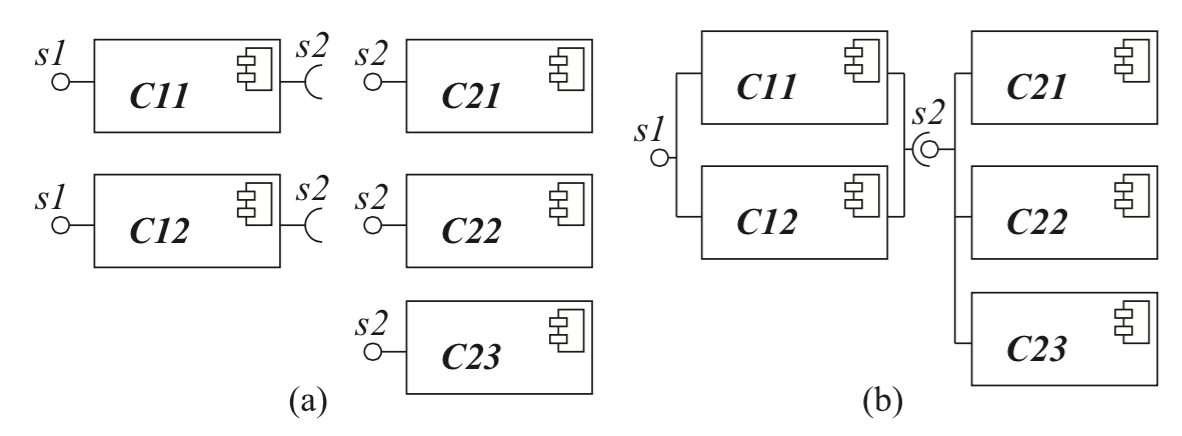
\includegraphics[width=\textwidth]{img/fig1.png}
\caption{Beispiel Component-and-Connector Ansicht}
\end{figure}

\note {
\begin{itemize}
\item Der Ansatz basiert auf einer Component-and-Connector Ansicht, da sie allgemein verwendet wird um über die Qualitätswerte zur Laufzeit zu reden.
\item Sockets für benötigte und angebotene Dienste
\item Gemeinsame Linien zeigen an dass mehrere Komponenten den gleichen Dienst anbieten oder benötigen.
\end{itemize}
}}

\section{Metriken}
\frame{\frametitle{Metriken}
\begin{Definition}[$UC_i $]
Komponenten, die den Dienst i bereitstellen
\end{Definition}

\begin{Definition}[$C_i $]
Komponenten, die den Dienst i bereitstellen können
\end{Definition}
}

\frame{\frametitle{Metriken}
\begin{figure}[h]
\centering
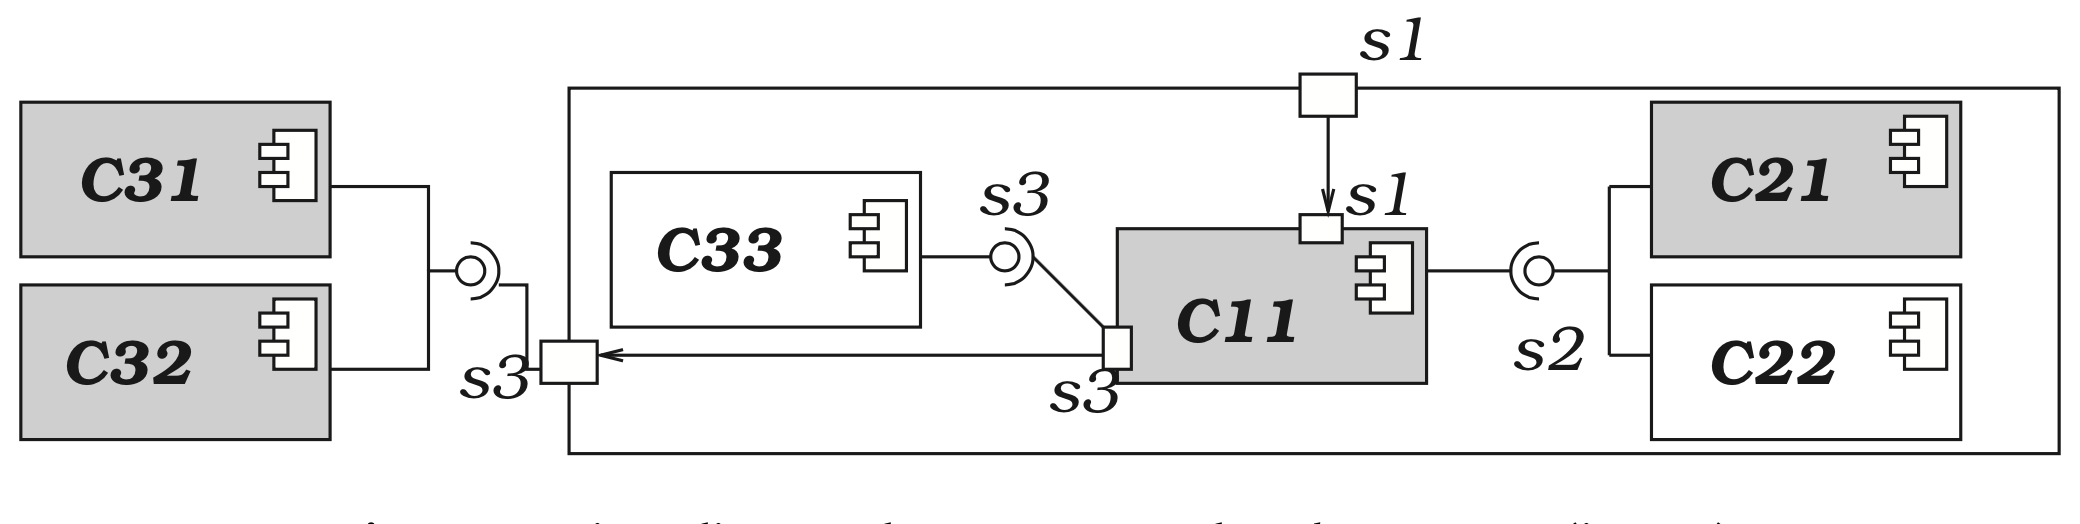
\includegraphics[width=\textwidth]{img/fig2.png}
\caption{Beispielarchitektur}
\end{figure}
}

\frame{\frametitle{Metriken}
\begin{itemize}
\item AAS und RAS
\item MAAS und MRAS
\item LSA
\end{itemize}
}

\subsection{AAS und RAS}
\frame{\frametitle{AAS}

\begin{Definition}[Absolute adaptability of a service]
$AAS_i = | UC_i | $
\end{Definition}

\begin{figure}[h]
\centering
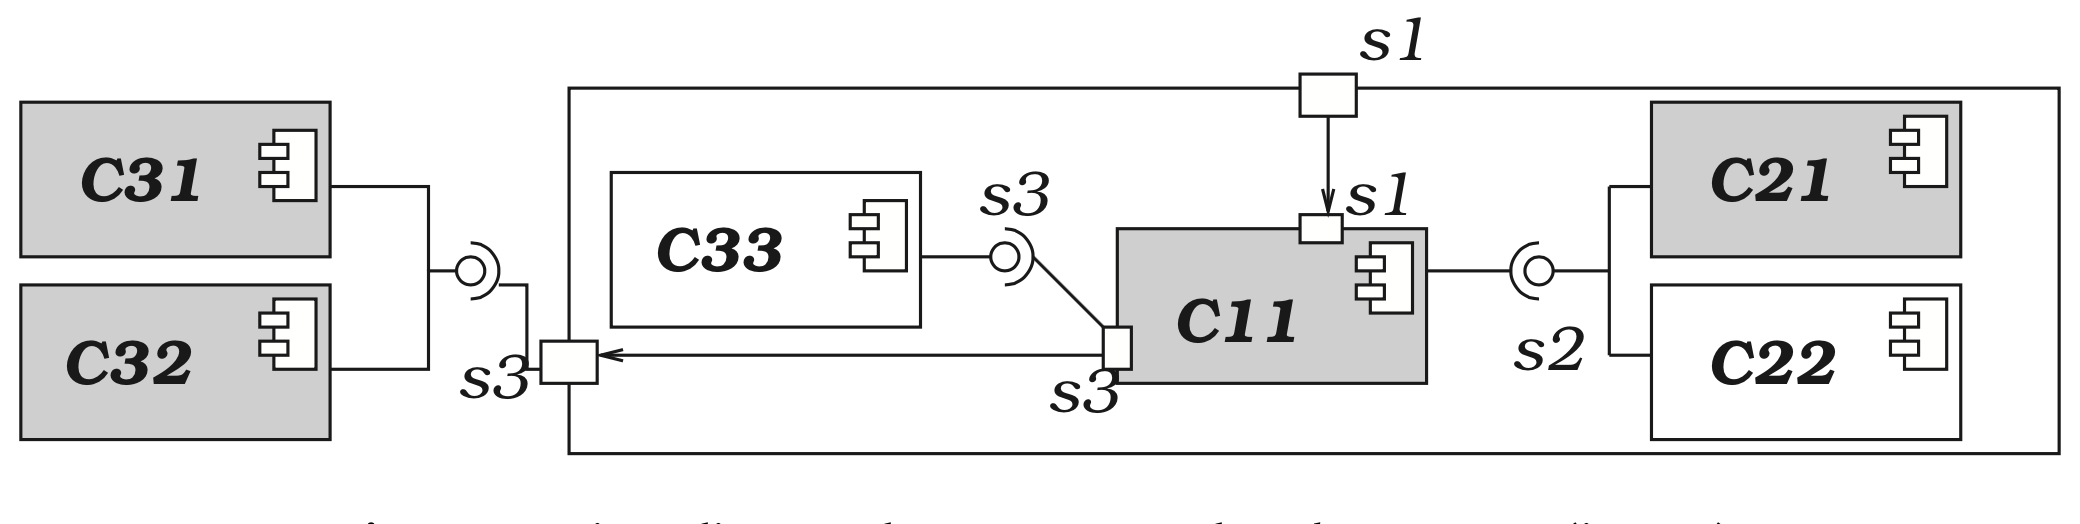
\includegraphics[width=\textwidth]{img/fig2.png}
\end{figure}

\note {
\begin{itemize}
\item \textbf{AAS} misst die Anzahl der benutzten Komponenten, welche gewisse Dienste bereitstellen.
\item Lösung: [1,1,2]
\end{itemize}
}}

\frame{\frametitle{RAS}
\begin{Definition}[Relative adaptability of a service]
$RAS_i = \frac{| UC_i |}{| C_i |}$
\end{Definition}

\begin{figure}[h]
\centering
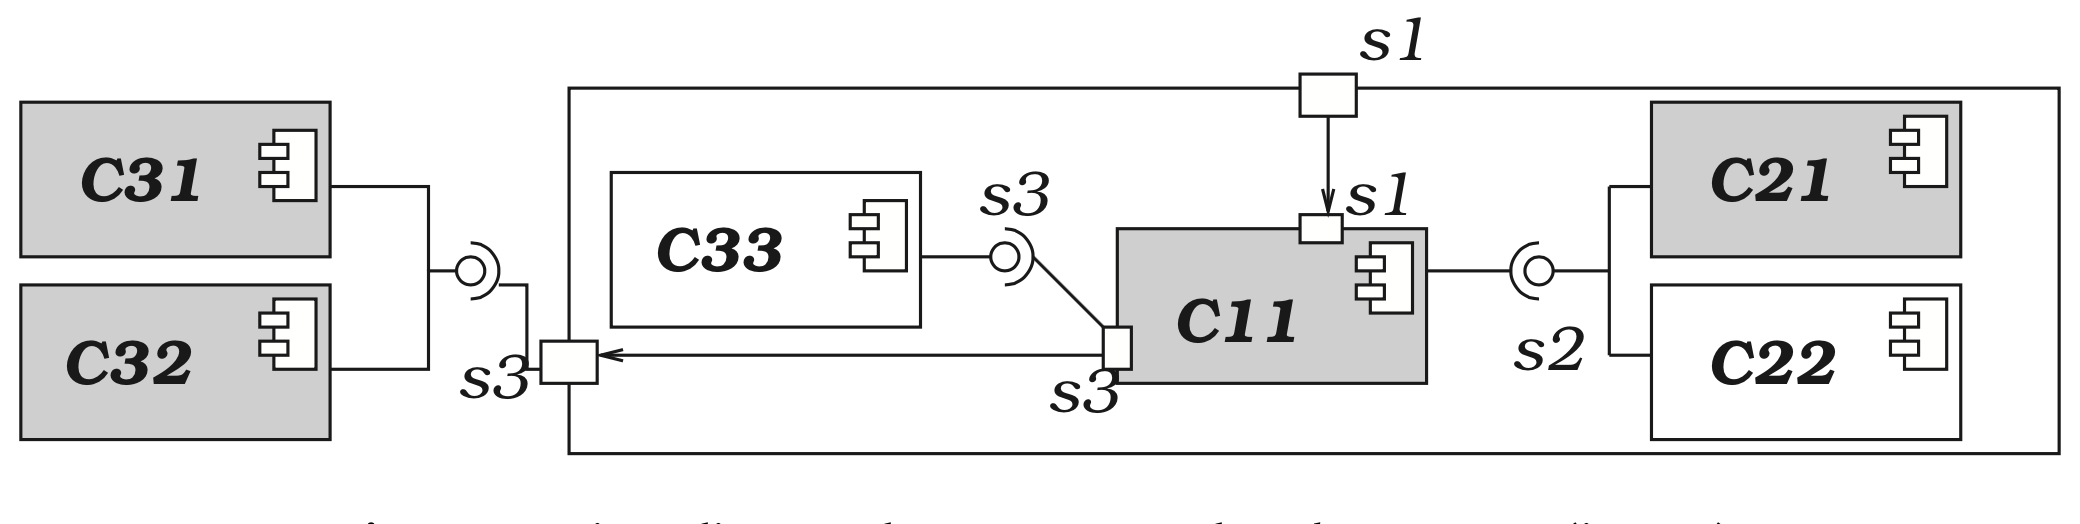
\includegraphics[width=\textwidth]{img/fig2.png}
\end{figure}

\note {
\begin{itemize}
\item \textbf{RAS} misst die Anzahl der verwendeten Komponenten, welche einen gegebenen Service bereitstellen in hinsicht auf die Anzahl der Komponenten, die tatsächlich solchen Service anbieten.
\item Lösung: [1,0.5, 0.6]
\end{itemize}
}}

\subsection{MAAS und MRAS}
\frame{\frametitle{MAAS}

\begin{Definition}[Mean of absolute adaptability of service]
$MAAS = \frac{\sum_{i=1}^n AAS_i }{n}$
\end{Definition}

\begin{figure}[h]
\centering
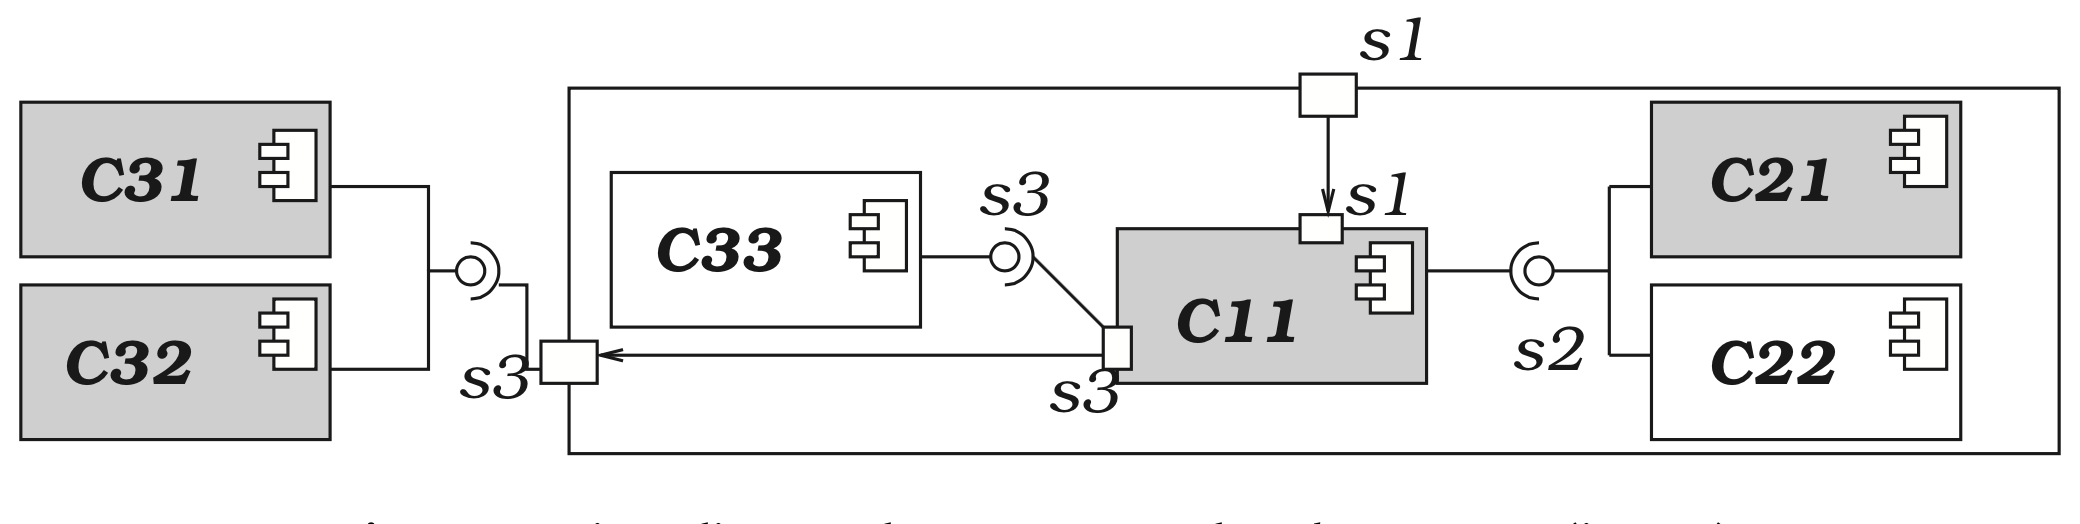
\includegraphics[width=\textwidth]{img/fig2.png}
\end{figure}

\note {

\begin{itemize}
\item \textbf{MAAS} misst die durchnittliche Anzahl der genutzten Komponenten pro Dienstleistung. Komponenten, die tatsächlich solchen Service anbieten.
\item Lösung: 4/3 = 1.3
\end{itemize}
}}

\frame{\frametitle{MRAS}

\begin{Definition}[Mean of relative adaptability of service]
$MAAS = \frac{\sum_{i=1}^n RAS_i }{n}$
\end{Definition}

\begin{figure}[h]
\centering
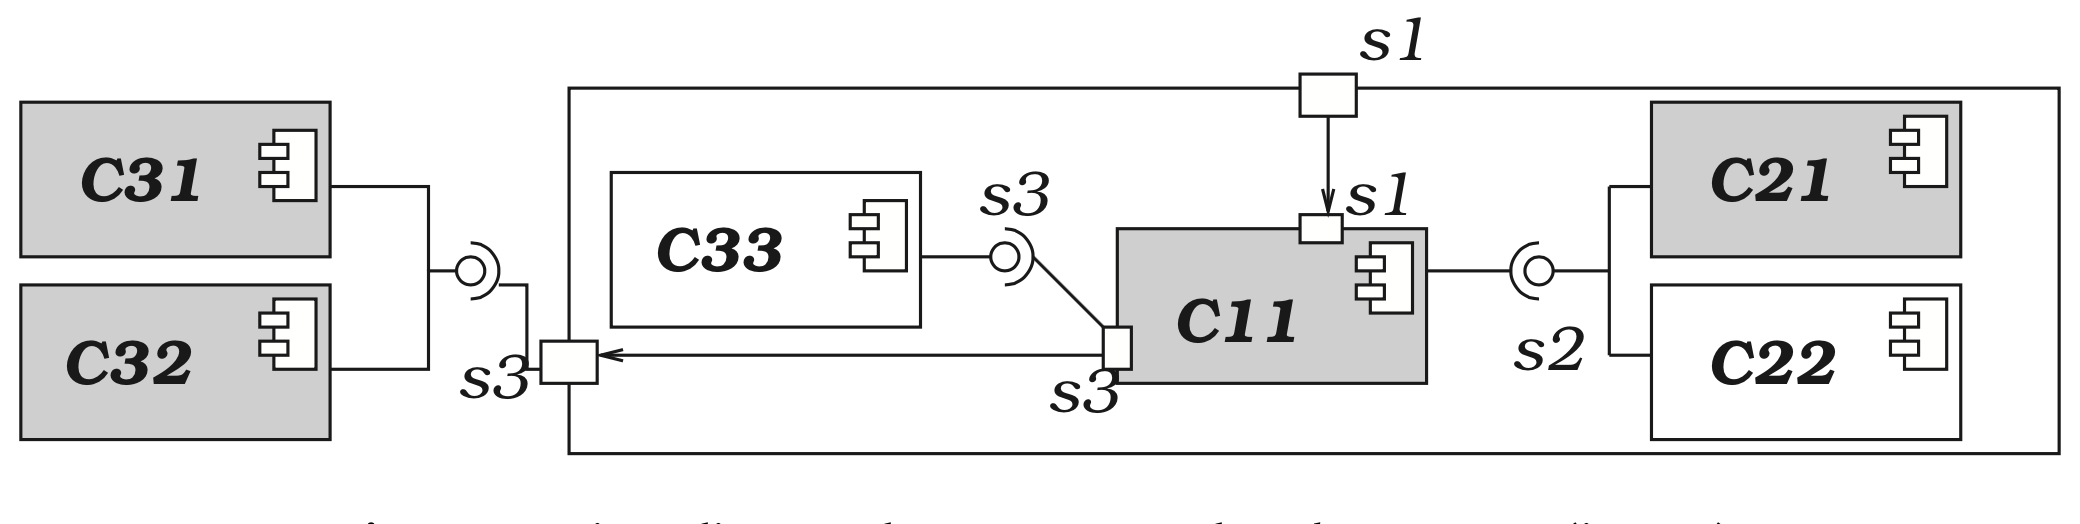
\includegraphics[width=\textwidth]{img/fig2.png}
\end{figure}

\note{
\begin{itemize}
\item \textbf{MRAS} misst den Durchschnitt des RAS (Relative Adaptability of a service).
\item Lösung: (1 + 0.5 + 0.6) / 3 = 0.7
\end{itemize}
}}

\subsection{LSA}
\frame{\frametitle{LSA}

\begin{Definition}[Level of system adaptability]
$LSA = \frac{\sum_{i=1}^n AAS_i }{\sum_{i=1}^n |C|}$
\end{Definition}

\begin{figure}[h]
\centering
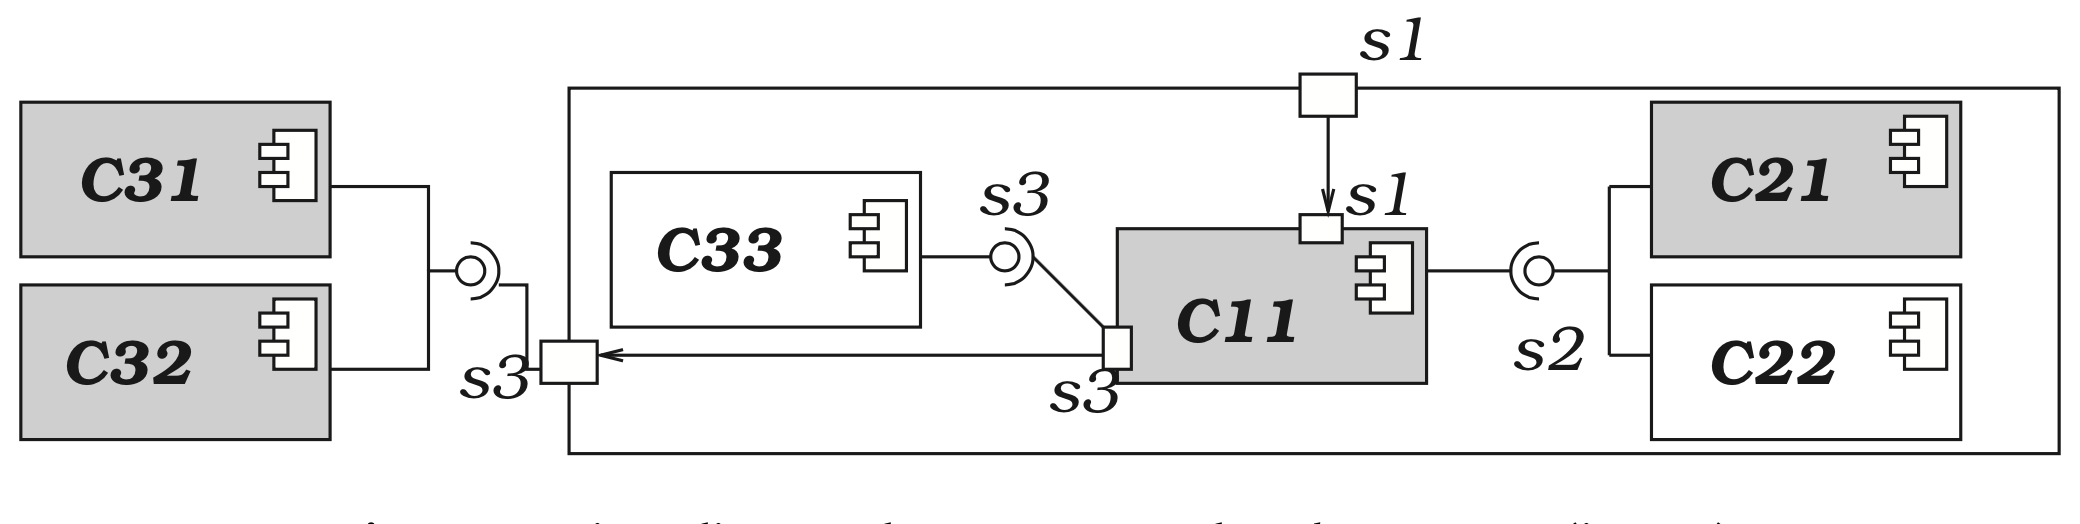
\includegraphics[width=\textwidth]{img/fig2.png}
\end{figure}

\note{
\begin{itemize}
\item \textbf{LSA} bezeichnet das Verhältnis zwischen der Anzahl an Komponenten aus denen ein System besteht und der Anzahl die das Anpassungsfähigste nutzen würde.
\item Lösung: 4 / (1 + 2 + 3)  = 0.66666
\end{itemize}
}}

\section{Ansatz}
\subsection{Adapt \textsuperscript{-} und Adapt \textsuperscript{+}}
\frame{\frametitle{Adapt \textsuperscript{-} und Adapt \textsuperscript{+}}
\begin{Definition}[$Adapt^-$]
Das niedrigste $A_i$ für welches man eine Architektur finden kann, welche die Anforderungen erfüllt.
\end{Definition}
\note {
\begin{itemize}
\item Anforderungen werden durch Architekten gewählt und beziehen sich auf QoS des Systems.
\item $A_i$ sind zunehmende Werte für die gewählte Metrik der Anpassungsfähigkeit.
\end{itemize}

}}

\frame{\frametitle{Adapt \textsuperscript{-} und Adapt \textsuperscript{+}}
\begin{Definition}[$Adapt^+$]
Das niedrigste $A_i$ für dessen Grenzen $Q_{A_{i}U}$ und $Q_{A_{i}L}$ die Anforderungen erfüllen.
\end{Definition}

\note {
\begin{itemize}
\item $Q_{A_{i}U}$ ist der höchste Qualitätswert den eine Architektur für ein Anpassungsfähigkeitsniveau erreichen kann.
\item $Q_{A_{i}U}$ ist entsprechend der niedrigste.
\end{itemize}
}}

\frame{\frametitle{Adapt \textsuperscript{-} und Adapt \textsuperscript{+}}

\begin{figure}[h]
\centering
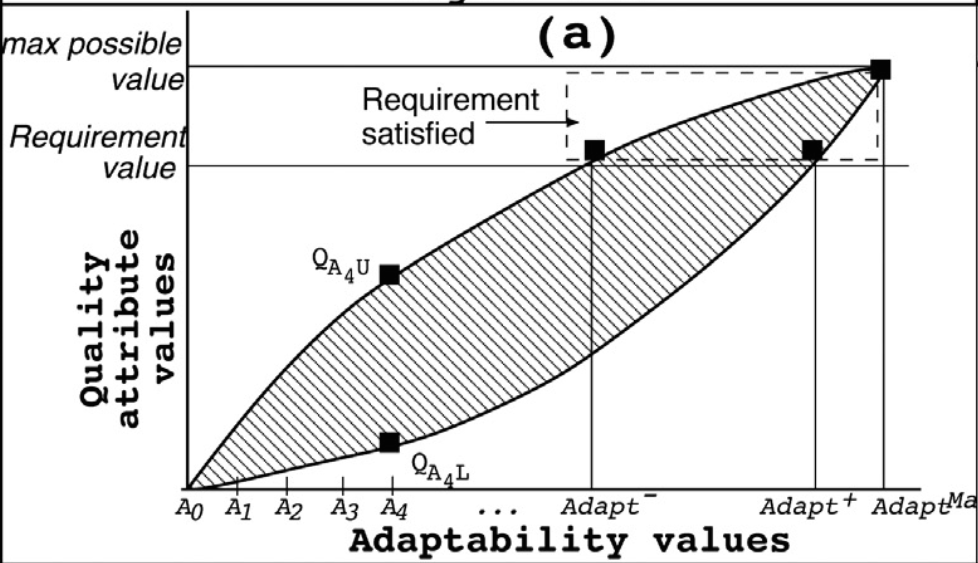
\includegraphics[width=\textwidth]{img/fig4_1.png}
\end{figure}

\note{
\begin{itemize}
\item  In (a) und (d) ist Adapt- das niedrigestes $A_i$ für welches man eine Architektur finden kann, welche die Anforderungen erfüllt. Adapt+ ist das niedrigste $A_i$, dessen Grenzen $Q_{A_i U}$ und $Q_{A_i L}$ die Anforderungen erfüllt.
\item  Die Werte zeigen, dass die Erfüllung der Anforderungen eine Anpassungsfähigkeit von Adapt- voraussetzen und, dass jede Architektur die mindestens Adapt+ hat die Anforderungen auch erfüllt. Für Anpassungsfähigkeit dazwischen gibt es Architekturen, die die Anforderungen erfüllen und solche die es nicht tun.
\end{itemize}
}}

\frame{\frametitle{Adapt \textsuperscript{-} und Adapt \textsuperscript{+}}

\begin{figure}[h]
\centering
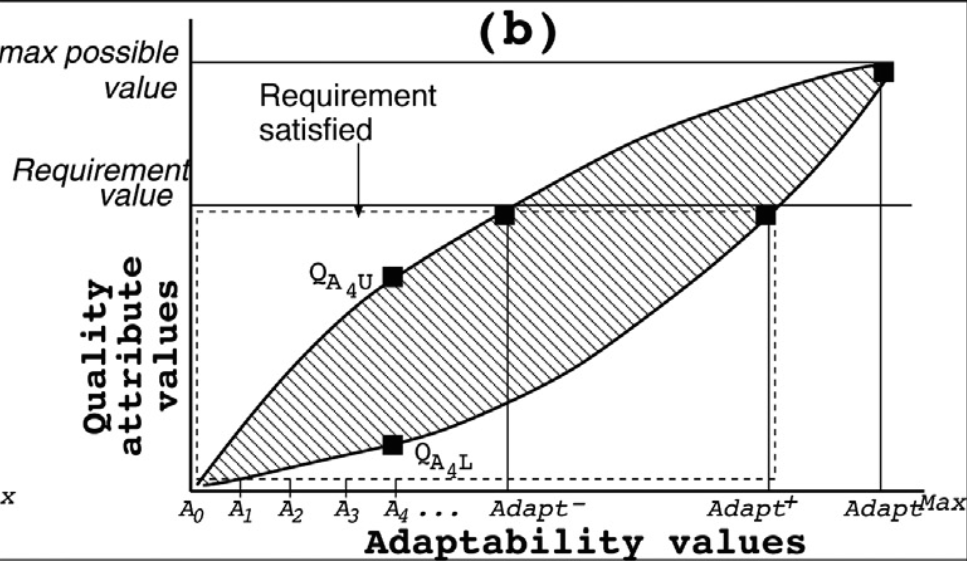
\includegraphics[width=\textwidth]{img/fig4_2.png}
\end{figure}

\note{
\begin{itemize}
\item  In (a) und (d) ist Adapt- das niedrigestes $A_i$ für welches man eine Architektur finden kann, welche die Anforderungen erfüllt. Adapt+ ist das niedrigste $A_i$, dessen Grenzen $Q_{A_i U}$ und $Q_{A_i L}$ die Anforderungen erfüllt.
\item  Die Werte zeigen, dass die Erfüllung der Anforderungen eine Anpassungsfähigkeit von Adapt- voraussetzen und, dass jede Architektur die mindestens Adapt+ hat die Anforderungen auch erfüllt. Für Anpassungsfähigkeit dazwischen gibt es Architekturen, die die Anforderungen erfüllen und solche die es nicht tun.
\end{itemize}
}}

\frame{\frametitle{Adapt \textsuperscript{-} und Adapt \textsuperscript{+}}

\begin{figure}[h]
\centering
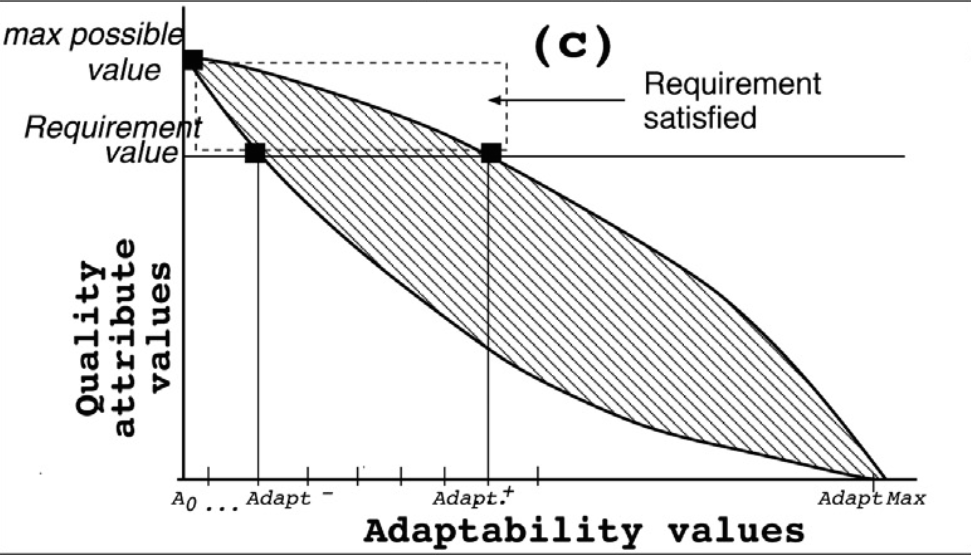
\includegraphics[width=\textwidth]{img/fig4_3.png}
\end{figure}

\note{
\begin{itemize}
\item  In (a) und (d) ist Adapt- das niedrigestes $A_i$ für welches man eine Architektur finden kann, welche die Anforderungen erfüllt. Adapt+ ist das niedrigste $A_i$, dessen Grenzen $Q_{A_i U}$ und $Q_{A_i L}$ die Anforderungen erfüllt.
\item  Die Werte zeigen, dass die Erfüllung der Anforderungen eine Anpassungsfähigkeit von Adapt- voraussetzen und, dass jede Architektur die mindestens Adapt+ hat die Anforderungen auch erfüllt. Für Anpassungsfähigkeit dazwischen gibt es Architekturen, die die Anforderungen erfüllen und solche die es nicht tun.
\end{itemize}
}}

\frame{\frametitle{Adapt \textsuperscript{-} und Adapt \textsuperscript{+}}

\begin{figure}[h]
\centering
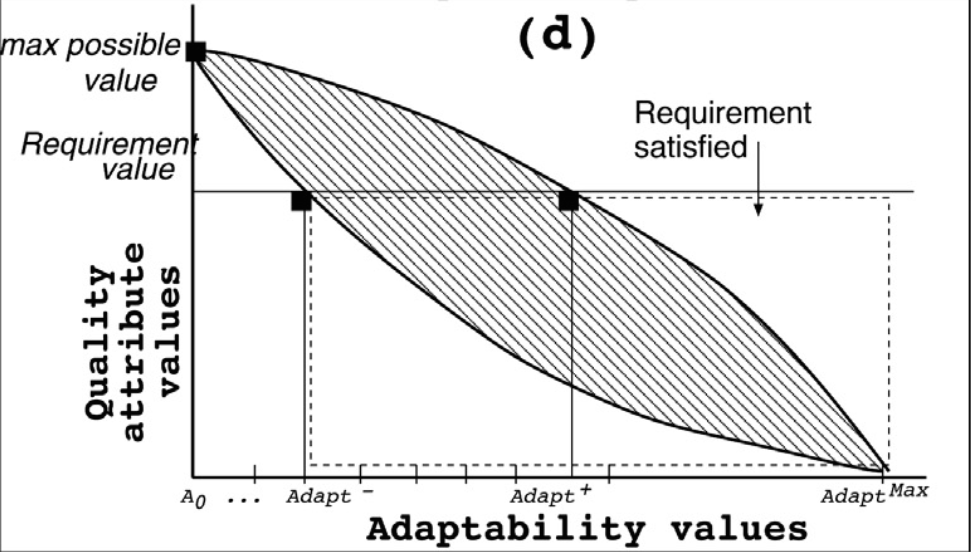
\includegraphics[width=\textwidth]{img/fig4_4.png}
\end{figure}

\note{
\begin{itemize}
\item  In (a) und (d) ist Adapt- das niedrigstes $A_i$ für welches man eine Architektur finden kann, welche die Anforderungen erfüllt. Adapt+ ist das niedrigste $A_i$, dessen Grenzen $Q_{A_i U}$ und $Q_{A_i L}$ die Anforderungen erfüllt.
\item  Die Werte zeigen, dass die Erfüllung der Anforderungen eine Anpassungsfähigkeit von Adapt- voraussetzen und, dass jede Architektur die mindestens Adapt+ hat die Anforderungen auch erfüllt. Für Anpassungsfähigkeit dazwischen gibt es Architekturen, die die Anforderungen erfüllen und solche die es nicht tun.
\end{itemize}
}}

\subsection{Mehrere Anforderungen}
\frame{\frametitle{Mehrere Anforderungen}

\begin{figure}[h]
\centering
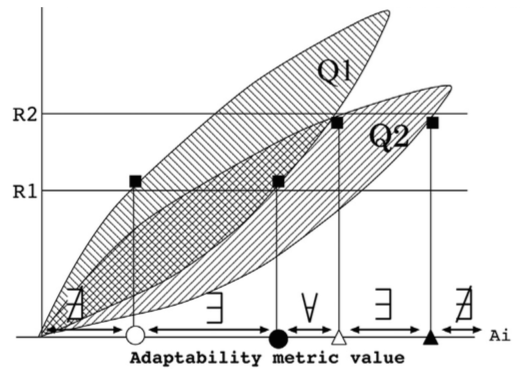
\includegraphics[width=0.75\textwidth]{img/fig7_1.png}
\end{figure}

\note {
\begin{itemize}
\item Es lassen sich bei Nutzung der gleichen Metrik zwei QoS in einen Graphen einzeichnen. Hierbei wird eine Fläche eingezeichnet, die die Werte bei allen möglichen Architekturen anzeigt. Es lassen sich Adapt+ und Adapt- für beide Qualitätsattribute einzeichnen, so entstehen (vielleicht) Bereiche in denen beide Anforderungen erfüllt sind, nur einer erfüllt ist oder keiner erfüllt ist.
\end{itemize}
}}

\frame{\frametitle{Mehrere Anforderungen}

\begin{figure}[h]
\centering
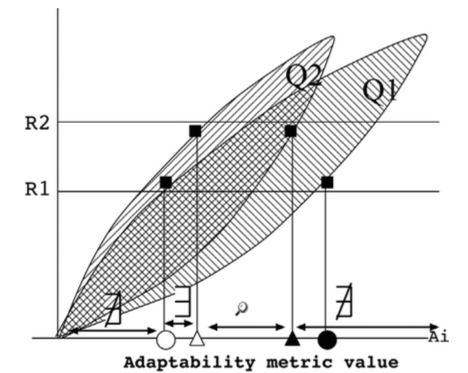
\includegraphics[width=0.75\textwidth]{img/fig7_2.png}
\end{figure}

\note {
\begin{itemize}
\item Es lassen sich bei Nutzung der gleichen Metrik zwei QoS in einen Graphen einzeichnen. Hierbei wird eine Fläche eingezeichnet, die die Werte bei allen möglichen Architekturen anzeigt. Es lassen sich Adapt+ und Adapt- für beide Qualitätsattribute einzeichnen, so entstehen (vielleicht) Bereiche in denen beide Anforderungen erfüllt sind, nur einer erfüllt ist oder keiner erfüllt ist.
\end{itemize}
}}

\subsection{Beziehungen der QoS zur Anpassungsfähigkeit}
\frame{\frametitle{Beziehungen der QoS zur Anpassungsfähigkeit}
\begin{figure}[h]
\centering
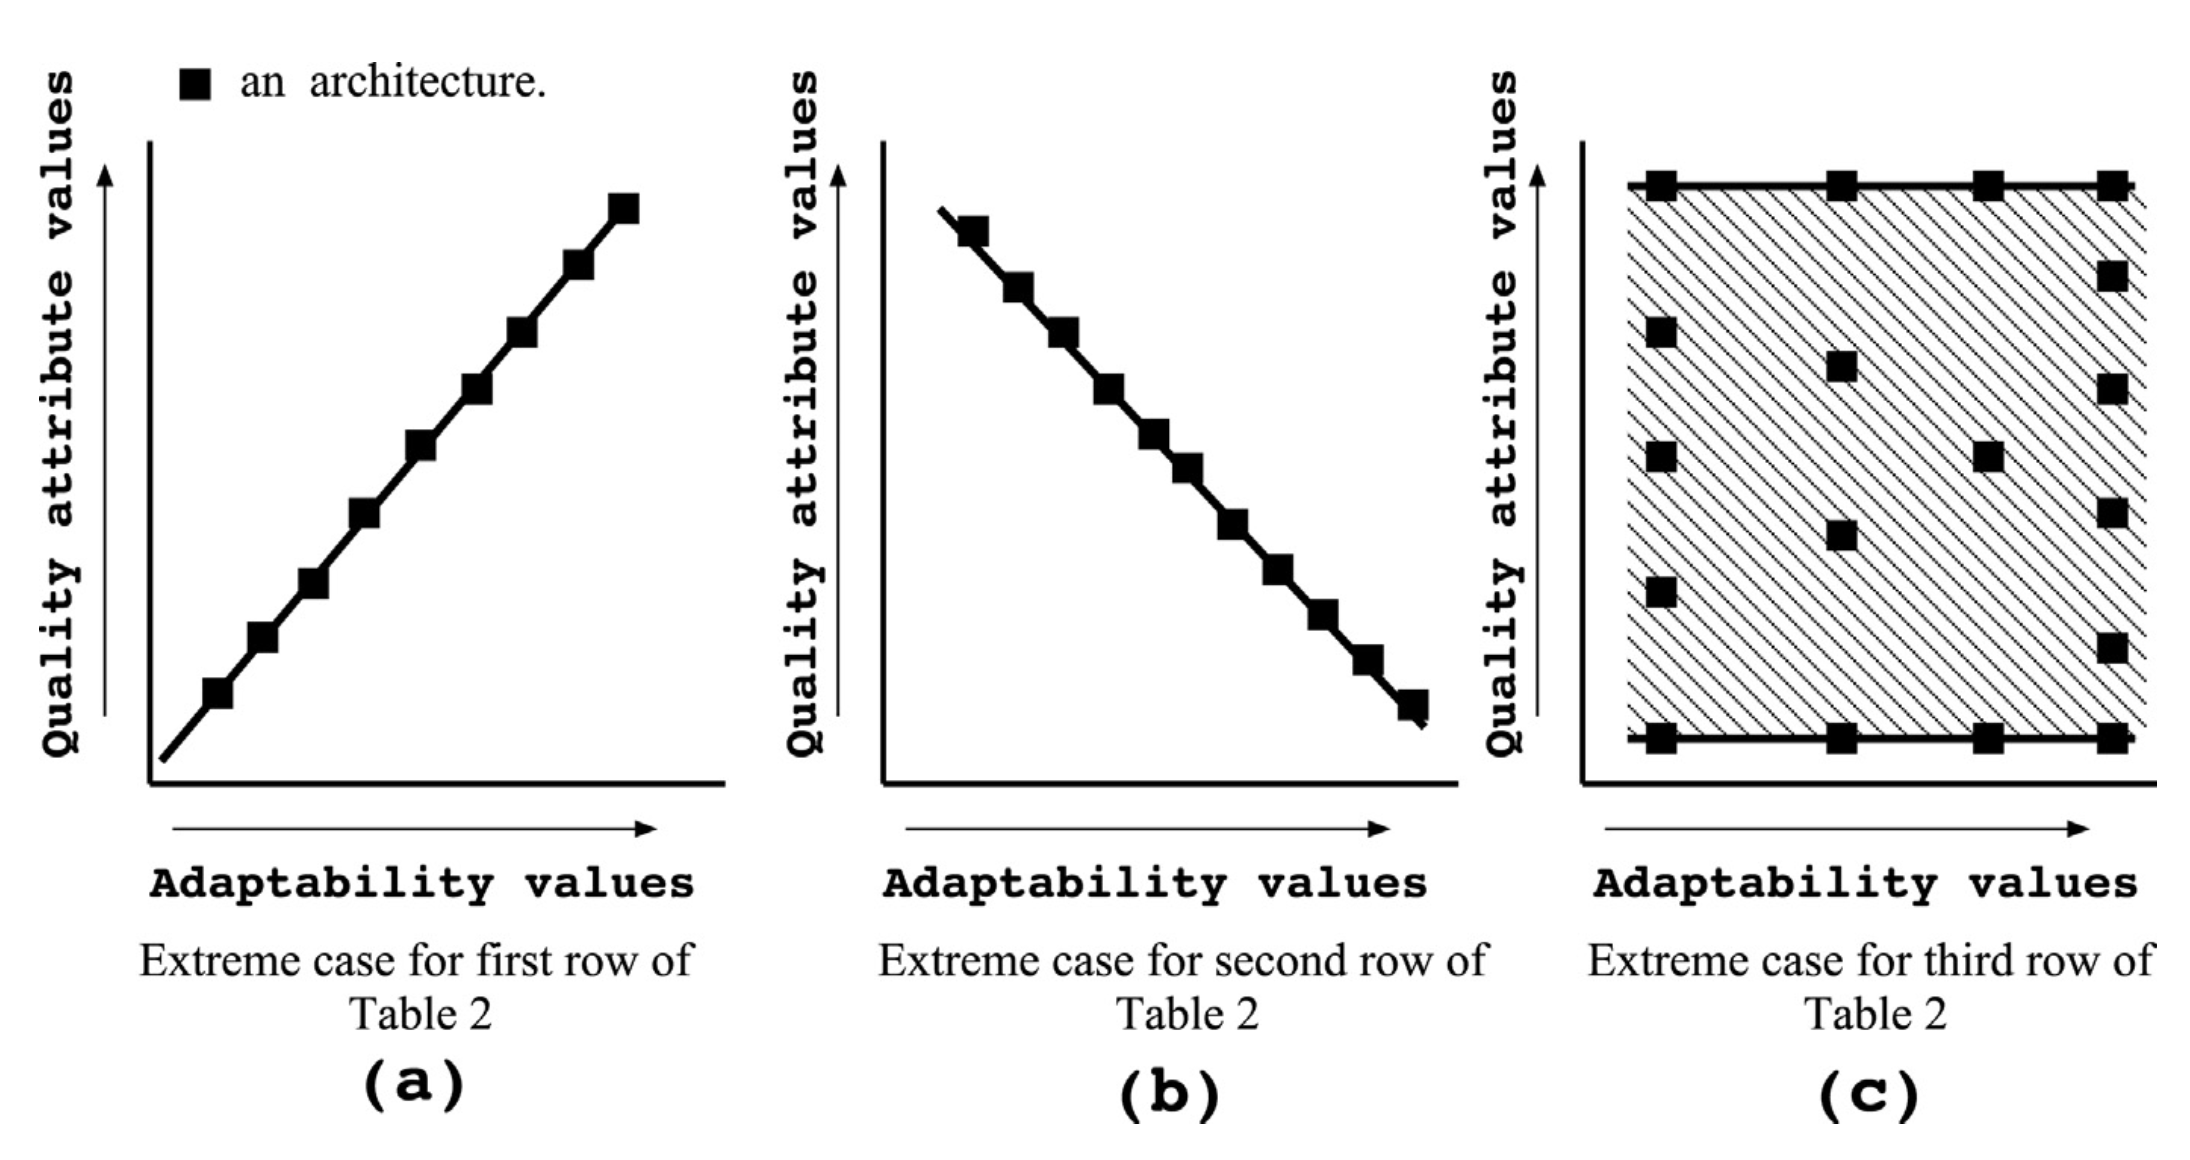
\includegraphics[width=\textwidth]{img/fig3.png}
\end{figure}

\note {
\begin{itemize}
\item Für jedes System gelten unterschiedliche Beziehungen zwischen QoS und Anpassungsfähigkeit
\item Wissen über die Beziehungen ermöglicht es den besten Kompromiss zu finden zwischen Anpassungsfähigkeit und Zielanforderung
\item Ziel der Analyse ist es zu zeigen, dass es eine Reihe von Möglichkeiten gibt ein System durch die Anwendung des Ansatzes zu entwerfen, welches die Anforderungen erfüllt und manchmal auch die gesamte Qualität und / oder Anpassbarkeit verbessert
\item SOLAR (SOftware quaLities and Adaptability Relationships) ist ein Programm, welches den Ansatz umsetzt. Es hat jedoch performance probleme (bei 30 komponenten bis zu 20 minuten)
\end{itemize}
}}

\section{Analyse des Ansatzes}

\frame{\frametitle{Vorteile}

\begin{itemize}
\item hilft die Architekturentscheidung zu rechtfertigen.
\item dauert länger als bisherige Verfahren, aber das Resultat ist auch bei Änderungen weiterhin nutzbar.
\end{itemize}

\note {
\begin{itemize}
\item \textbf{Ziel:} Zu zeigen, dass es eine Reihe von Möglichkeiten gibt mithilfe des Ansatzes ein System zu entwerfen, welches die Anforderungen erfüllt und manchmal auch die gesamte QoS und / oder Anpassbarkeit zu verbessern.
\item dauert länger als andere Ansätze, aber Erkenntnisse aus den anderen Ansätzen nutzlos sobald sich die Anforderungen ändern, hier nicht.
\item Es muss lediglich die Asymptote der Anforderungen neu gezeichnet werden und die neuen Komponenten entsprechend ausgewählt werden. 
\small{
\begin{itemize}
	\item neue Komponente: Ja, da es neue Möglichkeiten gibt
	\item Komponente zerstört: Ja, wenn in Architektur 
	\item Komponente ändert QoS: Wenn es in der Architektur ist bei Verschlechterung Ja, ansonsten nein. Falls es nicht in der Architektur ist sollte er angewendet werden.
	\item Die Anforderungen ändern sich: Wenn die Anforderungen strikter werden und die Anforderungen nicht mehr eingehalten muss der Ansatz genutzt werden, ansonsten nicht.
\end{itemize}
}
\end{itemize}
}}

\frame{\frametitle{Beschränkungen}

\begin{itemize}
\item Weicher Erfüllungsgrad kann mit dem aktuellen Ansatz nicht vereint werden, da $Adapt^+$ und $Adapt-$ in einem durchgehenden Erfüllbarkeitsschema nicht existieren würden
\item Keine Gewichtung von Komponenten \& Services
\item Fehlendes Wissen über die tatsächliche Umgebung und die Schwierigkeit bei der Definition architektureller Parameter
\end{itemize}

\note {
\begin{itemize}
\item Es wird für den Ansatz generell nur eine binäre Erfüllung der Anforderungen genutzt (erfüllt, nicht erfüllt). Eine weichere Form kann mit dem aktuellen Ansatz nicht vereint werden, da Adapt+ und Adapt- in einem durchgehenderen Erfüllbarkeitsschema nicht existieren würden
\item Bisher gibt es keine Gewichtung in der einige Komponenten, bzw Services wichtiger sein können als andere (WIP).
\item Normale Probleme (lack of knowledge about the real world execution enviroment and consequently the difficulty in defining architecture parameters)
\end{itemize}
}
}

\nocite{*}
\begingroup
\frame{\frametitle{Literatur}
\printbibliography
}
\endgroup

\end{document}